\documentclass[UTF-8,twoside,cs4size]{ctexart}
\usepackage[dvipsnames]{xcolor}
\usepackage{amsmath}
\usepackage{amssymb}
\usepackage{geometry}
\usepackage{setspace}
\usepackage{xeCJK}
\usepackage{ulem}
\usepackage{pstricks}
\usepackage{pstricks-add}
\usepackage{bm}
\usepackage{mathtools}
\usepackage{breqn}
\usepackage{mathrsfs}
\usepackage{esint}
\usepackage{textcomp}
\usepackage{upgreek}
\usepackage{pifont}
\usepackage{tikz}
\usepackage{circuitikz}
\usepackage{caption}
\usepackage{tabularx}
\usepackage{array}
\newcolumntype{Y}{>{\centering\arraybackslash}X}
\usepackage{pgfplots}
\usepackage{multirow}
\usepackage{pgfplotstable}
\usepackage{mhchem}
\usepackage{physics} % Add this package for \dt and \dif commands
\newcommand{\dif}{\mathrm{d}}
\usepackage{cases}
\usepackage{subfigure}
\usepackage{enumerate}
\usepackage{minipage-marginpar}
\usepackage{diagbox}
\usepackage{graphicx}


\graphicspath{{./figure/}}

\setCJKfamilyfont{zhsong}[AutoFakeBold = {5.6}]{STSong}
\newcommand*{\song}{\CJKfamily{zhsong}}

\geometry{a4paper,left=2cm,right=2cm,top=0.75cm,bottom=2.54cm}

\newcommand{\experiName}{热导与温度测量}%实验名称
\newcommand{\supervisor}{靳硕学}%指导教师
\newcommand{\name}{孙奕飞}
\newcommand{\studentNum}{2023k8009925001}
\newcommand{\class}{2}%班级
\newcommand{\group}{06}%组
\newcommand{\seat}{01}%座位号
\newcommand{\dateYear}{2024}
\newcommand{\dateMonth}{12}%月
\newcommand{\dateDay}{17}%日
\newcommand{\room}{教427}%地点
\newcommand{\others}{$\square$}

\ctexset{
    section={
        format+=\raggedright\song\large
    },
    subsection={
        name={\quad,.}
    },
    subsubsection={
        name={\qquad,.}
    }
}

\begin{document}
\noindent

\begin{center}

    \textbf{\song \zihao{-2} \ziju{0.5}《基础物理实验》实验报告}
    
\end{center}


\begin{center}
    \kaishu \zihao{5}
    \noindent \emph{实验名称}\underline{\makebox[28em][c]{\experiName}}
    \emph{指导教师}\underline{\makebox[9em][c]{\supervisor}}\\
    \emph{姓名}\underline{\makebox[6em][c]{\name}} 
    \emph{学号}\underline{\makebox[14em][c]{\studentNum}}
    \emph{分班分组及座号} \underline{\makebox[5em][c]{\class \ -\ \group \ -\ \seat }\emph{号}} \\
    \emph{实验日期} \underline{\makebox[3em][c]{\dateYear}} \emph{年}
    \underline{\makebox[2em][c]{\dateMonth}}\emph{月}
    \underline{\makebox[2em][c]{\dateDay}}\emph{日}
    \emph{实验地点}\underline{{\makebox[4em][c]\room}}
    \emph{调课/补课} \underline{\makebox[3em][c]{否}}
    \emph{成绩评定} \underline{\hspace{8em}}
    {\noindent}
    \rule[5pt]{17.7cm}{0.2em}
\end{center}

\section{实验目的}
\begin{enumerate}
    \item 通过实验掌握测定热导率的一种方法。
    \item 探究动态法的独特之处及其优越性能。
    \item 理解热波现象,进一步加深对波动理论的掌握。
    \item 借助电位差计测量热电偶的温差电动势。
    \item 运用平衡电桥获得热敏电阻与铜电阻的温度特性曲线。
    \item 设计非平衡电桥,用以完成对热敏电阻的实时测量。
\end{enumerate}

\section{实验仪器}
用绝热材料紧密包裹侧表面的圆柱形样品(本实验选择铜和铝作为两种测试材料),实验装置包括热电偶阵列(传感器)、脉冲热源与冷却设备、冷却水系统,DHT-2 型热学实验装置温度控制仪,UJ36a 型便携式直流电位差计,以及 DHQJ-5 型教学用多功能电桥。

\section{实验原理}
\subsection{动态法测量良导体热导率}
在样品上截取一小段圆柱体作为棒元,其示意图如图 (\ref{difx}) 所示。根据热传导定律,在单位时间内通过垂直于热量传播方向面积 $A$ 的热量(即热流量)表示为:
\[
\frac{\dif q}{\dif t} = -kA\frac{\dif T}{\dif x}
\]
其中,$k$ 是待测材料的热导率,$A$ 为截面积,$\frac{\dif T}{\dif x}$ 表示温度沿 $x$ 方向的梯度。

\begin{figure}[!h]
    \centering
    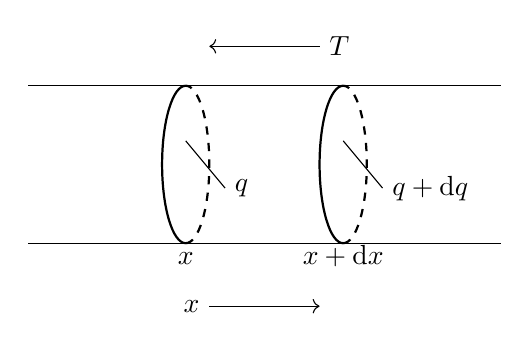
\begin{tikzpicture}
        \draw (0,0)--(6,0);
        \draw (0,2)--(6,2);
        \draw [thick] (2,2) arc (90:270:0.3 and 1);
        \draw [thick, dashed] (2,0) arc (-90:90:0.3 and 1);
        \draw [thick] (4,2) arc (90:270:0.3 and 1);
        \draw [thick, dashed] (4,0) arc (-90:90:0.3 and 1);
        \draw [<-] (2.3,2.5)--(3.7,2.5) node[right]{$ T $};
        \draw [->] (2.3,-0.8) node[left]{$ x $}--(3.7,-0.8);
        \node [below] at(2,0) {$ x $};
        \node [below] at(4,0.1) {$ x+\dif x $};
        \draw (2,1.3)--(2.5,0.7) node[right]{$ q $};
        \draw (4,1.3)--(4.5,0.7) node[right]{$ q+\dif q $};
    \end{tikzpicture}
    \caption{棒元结构示意图}
    \label{difx}
\end{figure}

对上述公式两边进行坐标微分,可得:
\[
\frac{\dif^2 q}{\dif x\dif t} = -kA \frac{\dif^2 T}{\dif x^2}\,\Longrightarrow\,\dif\frac{\dif q}{\dif t} = -kA\frac{\dif^2 T}{\dif x^2}.
\]

根据能量守恒定律,对于棒元在任意时刻的热平衡方程,我们有:
\[
C\rho A\dif x\frac{\dif T}{\dif t} = \dif\frac{\dif q}{\dif t} = -kA \frac{\dif^2 T}{\dif x^2} \dif x,
\]
其中,$C$ 和 $\rho$ 分别是材料的比热容与密度。由此可以得到热流方程:
\[
\frac{\dif T}{\dif t} = D \frac{\dif^2 T}{\dif x^2},
\]
其中 $D = \frac{k}{C\rho}$ 被称为热扩散系数。该方程的解描述了各点温度随时间的变化,其具体形式依赖于边界条件。若设热端的温度随时间呈简谐变化,即:
\[
T = T_0 + T_m\sin\omega t,
\]
而另一端通过冷水保持恒定低温 $T_0$,则方程的解(即棒中各点的温度分布)为:
\[
T = T_0 - \alpha x + T_m\exp\left(-\sqrt{\frac{\omega}{2D}}x\right)\sin\left(\omega t - \sqrt{\frac{\omega}{2D}}x\right),
\]
其中 $T_0$ 为直流成分,$\alpha$ 为线性成分斜率。从上式可以得出以下重要结论:

\begin{itemize}
    \item \kaishu (a) 当热端 $(x=0)$ 处的温度发生简谐变化时,该变化以衰减波的形式沿棒传播,这称为热波;
    \item \kaishu (b) 热波的传播速度为 $v = \sqrt{2D\omega}$;
    \item \kaishu (c) 热波波长为 $\lambda = 2\pi\sqrt{\frac{2D}{\omega}}$。
\end{itemize}

因此,在已知热端温度变化的角频率 $\omega$ 的条件下,通过测量热波的传播速度或波长即可求出热扩散系数 $D$。进而通过公式 $D=\frac{k}{C\rho}$ 推导出材料的热导率 $k$。

本实验利用公式 $v = \sqrt{2D\omega}$,可以推得:
\[
v^2 = 2\frac{k}{C\rho}\omega \,\Longrightarrow\, k = \frac{v^2C\rho}{4\pi f} = \frac{v^2C\rho}{4\pi} T,
\]
其中 $f$ 和 $T$ 分别为热端温度简谐变化的频率与周期。要实现上述测量,需确保热量在样品中呈一维传播状态,同时热端温度的变化符合简谐规律。

\subsection{温度的测量和温度计的设计}
\subsubsection{用电位差计测量热电偶的温差电动势}

热电偶,又称温差电偶,是由 A 和 B 两种不同金属材料的导线构成,其端点紧密连接形成闭合回路。当两个接点的温度分别为 $t$ 和 $t_0$ 时,回路中会产生直流电动势,这一电动势被称为温差电动势或热电动势。若热电偶的材质一定,温差电动势 $E_x$ 仅随两个接点温度变化,并在一定温度范围内近似满足:
\[
E_x \approx \alpha (t - t_0),
\]
其中 $\alpha$ 称为温差电系数,其数值由热电偶的金属材料决定。

要测量温差电动势,需要将热电偶连接到电位差计上。为了确保测量过程中热电偶的特性不受仪器引入的影响,实验需要遵循一定条件。根据伏打定律,如果在 A 和 B 两种金属间引入第三种金属 C,而其与 A 和 B 的两个接点保持在相同温度,则闭合回路的总温差电动势等于只由 A 和 B 两种金属构成回路时的电动势。

通常,热电偶由 A 和 B 两种非同质金属导线构成,其中一端焊接形成热端,另一端分别与铜引线焊接并形成两个冷端。铜引线与电位差计连接,形成热电偶温度计。

实验中将冷端放置于冰水混合物中以保持 $t_0 = 0 \, ^\circ \mathrm{C}$,而将热端置于待测温度环境中,通过测量温差电动势即可得到温度差。

\subsubsection{用平衡点桥测电阻的温度特性曲线}
\textbf{1.金属电阻温度计}

通常,金属电阻随温度的变化遵循以下关系式:
\[
R_x = R_{x0}(1+\alpha t + \beta t^2),
\]
其中 $R_{x0}$ 为 $t = 0 \, ^\circ \mathrm{C}$ 时的电阻值。例如,铜电阻的相关参数为:
\[
R_{x0} = 50 \, \Omega \qquad \alpha = 4.289 \times 10^{-3} \, ^\circ\mathrm{C}^{-1} \qquad \beta = 2.133 \times 10^{-7} \, ^\circ\mathrm{C}^{-2}.
\]

一般情况下,当温度较低时,可以忽略温度二次项 $\beta t^2$ 的贡献,此时金属电阻随温度的变化可近似看作线性关系,即:
\[
R_x = R_{x0}(1+\alpha t) = R_{x0} + \alpha t R_{x0}.
\]

实验中,可使用控温仪将铜电阻的温度稳定在一系列不同的温度点,在温度平稳后,通过平衡电桥测量出铜电阻的阻值,并绘制温度-阻值曲线。通过对数据进行线性拟合,可以求得温度系数 $\alpha$。

\textbf{2.半导体热敏温度计}

半导体热敏电阻(NTC)通常由一些金属氧化物(如 $ \mathrm{Fe_3O_4}$、$\mathrm{MgCr_2O_4}$ 等半导体)制成。在这些半导体材料中,自由电子的数量会随着温度的升高而迅速增加,从而显著提高导电能力。因此,NTC 热敏电阻具有负的电阻温度系数,其电阻值随温度的升高而迅速下降。此外,通过改良设计,还可以制成具有正温度系数的热敏电阻(简称 PTC)。

热敏电阻的电阻-温度特性可以用下列指数关系描述:
\[
R_T = A \mathrm{e}^{B/T},
\]
其中,$A$ 是一个与材料特性和电阻器几何形状相关的常数,$B$ 是一个与材料半导体特性相关的常数,$T$ 为绝对温度。

为了准确确定常数 $A$ 和 $B$,可以对上式取对数,得到:
\begin{equation}\label{2-3-2-2-1}
\ln R_T = \ln A + \frac{B}{T}.
\end{equation}

通过选择多个不同的温度点 $T$,可以测量对应的电阻值 $R_T$。

当 $T = T_1$ 时,上式写为:
\[
\ln R_{T_1} = \ln A + \frac{B}{T_1}.
\]

当 $T = T_2$ 时,上式为:
\[
\ln R_{T_2} = \ln A + \frac{B}{T_2}.
\]

将以上两式相减,可以得到:
\begin{equation}\label{2-3-2-2-2}
B = \frac{\ln R_{T_1} - \ln R_{T_2}}{\frac{1}{T_1} - \frac{1}{T_2}}.
\end{equation}

常见半导体热敏电阻的 $B$ 值通常介于 $1500 \sim 5000 \, \mathrm{K}$ 之间。

将式 (\ref{2-3-2-2-2}) 中的 $B$ 的表达式代入到式 (\ref{2-3-2-2-1}),可以求得 $A$:
\begin{equation}\label{2-3-2-2-3}
A = R_{T_1} \mathrm{e}^{-B/T_1}.
\end{equation}

实验时,可以使用控温仪将热敏电阻的温度控制在一系列不同的温度点上,通过平衡电桥测量对应的电阻值 $R_T$,并根据式 (\ref{2-3-2-2-1}) 进行线性拟合,以求出热敏电阻的常数 $A$ 和 $B$。如果仅测量两个温度点,则可以通过式 (\ref{2-3-2-2-2}) 和 (\ref{2-3-2-2-3}) 直接计算出 $A$ 和 $B$。

\textbf{3.设计非平衡电桥实现对热敏电阻的实时测量}

非平衡电桥的电路图如图所示:
\begin{figure}[!h]
    \centering
    \begin{circuitikz}
        \draw (0.8,0.5)
        to[short] (0,0)
        to[short,o-] (-2.5,0)
        to[short] (-2.5,3)
        to[short,-*] (-2,3)
        to[european resistor,-*,l={$ R_1 $},a={$ I_1 $}] (0,4.5)
        to[european resistor,-*,l={$ R_3 $},a={$ I_3 $}] (2,3);
        \draw (-2,3)
        to[european resistor,-*,l={$ R_2 $},a={$ I_2 $}] (0,1.5)
        to[european resistor,-*,l={$ R_x $},a={$ I_4 $}] (2,3);
        \draw (0,4.5)
        to[short] (0,5)
        to[short] (3,5)
        to[voltmeter,l={$ U_0 $}] (5,5)
        to[short] (5,1)
        to[short] (0,1)
        to[short] (0,1.5);
        \draw (0.9,0)
        to[battery,o-,a={$ E $}] (3,0)
        to[short] (3,3)
        to[short] (2,3);
        \node[below] at(0.45,0) {$ K $};
    \end{circuitikz}
    \caption{非平衡电桥电路图}
\end{figure}

非平衡电桥的测试步骤与平衡电桥类似,只是采用电压表测量电桥两端的电压 $U_0$,并假设电压表具有无穷大内阻,因此忽略电压表中的电流。平衡电桥的电压为 0,而非平衡电桥的电压 $U_0$ 则会随 $R_x$ 的变化而实时变化。通过计算合理选取 $R_1, R_2, R_3$ 和 $E$,使测试电压 $U_0$ 随温度 $t$ 线性变化,从而实现对温度的实时测量。

非平衡电桥的输出电压为:
\begin{equation}\label{2-3-3-1}
    U_0 = \left(\frac{R_x}{R_2 + R_x} - \frac{R_3}{R_1 + R_3}\right)E,
\end{equation}
其中
\begin{equation}\label{2-3-3-2}
    R_x = A \mathrm{e}^{B/T},
\end{equation}
而 $A, B$ 的值可以通过式 (\ref{eq:2-3-2-2-2}) 和 (\ref{eq:2-3-2-2-3}) 求得。

将式 (\ref{eq:2-3-3-2}) 代入式 (\ref{eq:2-3-3-1}),即可得到 $U_0$ 和 $T$ 的函数关系。对 $U_0$ 进行泰勒展开,忽略三阶及以上的高阶项,有:
\[
U_0 = U_{01} + U_0'(T - T_1) + U_0''(T - T_1)^2,
\]
其中 $T_1$ 是测试区间的中间温度值。例如,监测 $30 \sim 50$ \textcelsius 的温度区间,则可取 $T_1 = 40$ \textcelsius。若令 $U_0'' = 0$,可得:
\begin{equation}\label{eq:28}
    R_x = A \mathrm{e}^{B/T} = \frac{B + 2T}{B - 2T}R_2,
\end{equation}
进而得到 $U_0$ 关于 $T$ 的线性表达式:
\[
U_0 = \lambda + m(t - t_1),
\]
其中
\[
\lambda = \left(\frac{B + 2T_1}{2B} - \frac{R_3}{R_1 + R_3}\right)E = U_{01}, \quad 
m = \left(\frac{4T_1^2 - B^2}{4BT_1^2}\right)E = U_0',
\]
此处由绝对温度 $T$ 替换为摄氏温度 $t$。$\lambda$ 表示中间温度点对应的 $U_0$ 值,$m$ 是灵敏度。

通过已知的 $\lambda, m$ 和两个温度点,可以计算 $A, B$,并进一步利用式 (\ref{28}) 确定 $R_2, R_1/R_3$ 和 $E$。其具体表达式如下:
\[
E = \left(\frac{4BT_1^2}{4T_1^2 - B^2}\right)m, \quad 
R_2 = \frac{B - 2T}{B + 2T}R_{xT_1}, \quad 
\frac{R_1}{R_3} = \frac{2BE}{(B + 2T_1)E - 2B\lambda} - 1.
\]

根据计算结果,可以设定非平衡电桥的各参数,以满足实际测量需要。


\section{实验内容}
\subsection{动态法测量良导体热导率}
\begin{enumerate}
    \item 检查各连接管路是否畅通,确保无堵塞情况。随后打开水源,从出水口观察水流量,要求水流稳定。冷却水管在两个样品间为串联结构,水流方向为先通过铝样品后通过铜样品。因此,通常先测铜样品,再测铝样品,以避免冷却水温度升高对实验产生影响。
    
    \item 打开电源,启动仪器主机,使其进入工作状态。
    
    \item 打开操作软件,在控制界面中设置热源周期 $T = 180 \, \mathrm{s}$,并选择铜样品进行首次测量。
    
    \item 点击“操作”栏中的“测量”按钮,开始测量工作。仪器会实时在窗口上绘制 $T-t$ 曲线族。测量约 40 分钟后,系统达到动态平衡,样品内部温度进入动态稳定状态。此时,按下“暂停”按钮,并通过“文件”菜单保存测量得到的数据。
    
    \item 将样品更换为铝样品,然后重复步骤 4。
    
    \item 将实验所得数据通过网络发送至个人账户。最后,依次关闭测量仪器和计算机。
\end{enumerate}

\subsection{温度的测量和温度计的设计}
\subsubsection{用电位差计测热电偶的温差电动势}

\begin{enumerate}
    \item 在室温下测量并记录热电偶的电动势。
    
    \item 打开温控仪电源,对热端进行加热。在温度范围 $30 \sim 50 $\textcelsius 内,每隔 $5$\textcelsius 测量一组 $ (t, E_x) $ 数据。
    
    \item 绘制温度特性曲线,通过线性拟合计算并确定温度系数。
\end{enumerate}
\subsection{用平衡电桥测热敏电阻和铜电阻的电阻值}

\begin{enumerate}
    \item 在室温下测量并记录热敏电阻与铜电阻的电阻值。
    
    \item 在温度范围 $30 \sim 50 $\textcelsius 内,每隔 $5$\textcelsius 测量记录一组 $ (t, R_x) $ 数据。
    
    \item 绘制温度特性曲线,并通过线性拟合计算温度系数。
\end{enumerate}

\subsubsection{用非平衡电桥制作热敏电阻温度计}
\begin{enumerate}
    \item 选定 $\lambda = -400\,\mathrm{mV}, \; m = -10\,\mathrm{mV/\, ^\circ \mathrm{C}}, \; t_1 = 40 \, ^\circ \mathrm{C}$,根据在 $30 \, ^\circ \mathrm{C}$ 和 $50 \, ^\circ \mathrm{C}$ 下测得的热敏电阻阻值计算 $A, \, B$,进一步计算 $E, \, R_2, \, \frac{R_1}{R_3}$。
    
    \item 根据计算结果,设定非平衡电桥的参数。将温控仪的温度设定为 $40 \, ^\circ \mathrm{C}$,通过微调 $R_2$ 的阻值,使电压表测得的电压值接近 $-400\,\mathrm{mV}$。
    
    \item 改变温控仪的温度,在 $40 \sim 50 \, ^\circ \mathrm{C}$ 范围内,每隔 $2.5 \, ^\circ \mathrm{C}$ 测量一组 $U_0, \, t$ 数据,评估自制温度计的测温精度。
\end{enumerate}

\section{实验结果与数据处理}
\subsection{热波波速的测量}
相邻热电偶的距离为 $l_0=2\,\mathrm{cm}$,周期为 $T=180\,\mathrm{s}$。铜的比热容为 $0.385\,\mathrm{J/(g\cdot K)}$,密度为 $8.92\,\mathrm{g/cm^3}$;而铝的比热容是 $0.9\,\mathrm{J/(g\cdot K)}$,密度为 $2.7\,\mathrm{g/cm^3}$。\par
处理数据时,主要基于如下原则选取数据点:优先选择趋于稳定的曲线段,即曲线靠后的部分;选择距离较近的测量点进行分析;考虑到峰值可能对应多个时间点,需取其平均值作为最终结果。
\subsubsection{动态法测铜的热导率}
根据实验存储的数据,计算后得到如下结果:
\begin{table}[!h]
    \centering
    \renewcommand\arraystretch{1.5}
    ~\
    
    \caption{动态法测铜的热导率数据记录}
    
    \begin{tabularx}{\textwidth}{|c|Y|Y|Y|Y|Y|Y|}
        \hline
        测量点$ n $&0\,cm&2\,cm&4\,cm&6\,cm&8\,cm&10\,cm\\
        \hline
        对应峰值时间$ t(\mathrm s) $&2717.52&2710.52&2703.52&2696.40&2689.52&2682.04\\
        \hline
        波速(m/s)&0.002857&0.002857&0.00281&0.0029&0.00267&—\\
        \hline
    \end{tabularx}
\end{table}
由上可知,波速的平均值为
	\[\bar V = 0.0028188\,\mathrm{m/s}\]
	
	根据公式$ k=\frac{V^2C\rho}{4\pi f}=\frac{V^2C\rho T}{4\pi} $可求得铜的热导率为
        \[k_{\mathrm{Cu}}=\frac{V^2C\rho T}{4\pi}=397.22467\,\mathrm{W/(m\cdot\,^\circ \mathrm{C})}\]
    相对误差为$0.81 \%$。

\subsubsection{动态法测铝的热导率}
\begin{table}[!h]
	\centering
	\renewcommand\arraystretch{1.5}
	\caption{动态法测铝的热导率数据记录}
	\begin{tabularx}{\textwidth}{|c|Y|Y|Y|Y|Y|Y|}
		\hline
		测量点$ n $&0\,cm&2\,cm&4\,cm&6\,cm&8\,cm&10\,cm\\
		\hline
		对应峰值时间$ t(\mathrm s) $&1900.52&1905.52&1913.04&1923.04&1933.52&1941.52\\
		\hline
		波速(m/s)&0.00400&0.00266&0.00200&0.00191&0.00250&—\\
		\hline
	\end{tabularx}
	\end{table}
	那么波速的平均值为
	\(\bar V=0.00261\,\mathrm{m/s}\),
	所以可求得铝的热导率为
	\[k_{\mathrm{Al}}=\frac{V^2C\rho T}{4\pi}=231.84\,\mathrm{W/(m\cdot\,^\circ \mathrm{C})}\]
    相对误差为$2.177 \%$。
\subsubsection{误差分析}
总体来看,两实验测得的金属热导率与理论值相差不大,误差的可能来为:实验仪器本身的精确度存在一定限制,例如热水管可能与外界发生热量交换,导致加热不完全是稳定的正弦形式;此外,水流的速度与大小、以及铜样品的形状和性质随温度变化的影响,也会对测定结果造成干扰。

\subsection{温度的测量和温度计的设计}
\subsubsection{电位差计测热电偶的温差电动势}
实验过程中,将冷端置于冰水混合物中,以保持冷端的温度为 $0^\circ \mathrm{C}$。在室温 $t=27.9^\circ \mathrm{C}$ 下测得热电偶的电动势为 $E_x=0.58\,\mathrm{mV}$。

通过调整温度并记录实验数据,得到以下结果:

\begin{table}[!h]
    \centering
    \renewcommand\arraystretch{1.5}
	\caption{不同温度下热电偶的温差电动势}
    \begin{tabular}{|l|l|l|l|l|l|l|l|}
    \hline
        温度$t(^{\circ}C)$ & 30.5 & 35.8 & 39.8 & 44.9 & 50.1 \\ \hline
        电动势$E_x(mV)$ & 1.08 & 1.34 & 1.51 & 1.70 &1.89\\ \hline
    \end{tabular}
\end{table}
利用python中的Scipy库进行线性拟合,得到如下图像:
\begin{figure}[!h]
    \centering
    \includegraphics*[scale=0.7]{output.png}
    \caption{$E_x - t$温度曲线}
\end{figure}

由式$ E_x\approx\alpha(t-t_0) $可知上述拟合直线的斜率即为热电偶的温差电系数:
	\[\alpha = 0.0410\,\mathrm{mV/^\circ \mathrm{C}}\]

\subsubsection{平衡电桥测铜电阻温度特性曲线}
在室温$ t=27.5^\circ \mathrm{C}$下测得铜电阻阻值为$ R_x=56.7\,\Omega $。
	
调整温度,实验数据记录如下:
\begin{table}[!h]
    \centering
    \renewcommand\arraystretch{1.5}
	\caption{不同温度下铜电阻阻值}
    \begin{tabular}{|l|l|l|l|l|l|}
    \hline
        温度$t(^{\circ}C)$ & 30.5 & 35.8 & 39.8 & 44.9 & 50.1 \\ \hline
        铜电阻$R_x(\Omega)$ & 58.6 & 59.7 & 61.1 & 62.2 & 63.3 \\ \hline
    \end{tabular}
\end{table}	

利用python中的Scipy库进行线性拟合,得到如下图像:
\begin{figure}[!h]
    \centering
    \includegraphics*[scale=0.7]{output1.png}
    \caption{$R_x - t$温度特性曲线}
\end{figure}

由公式$ R_x=R_{x0}+\alpha tR_{x0} $可知:
\[R_{x0}=51.107\,\Omega,\quad \alpha=\frac{0.245}{51.107}^\circ \mathrm{C}^{-1}=0.00479^\circ \mathrm{C}^{-1}\]

\subsubsection{平衡点桥测热敏电阻温度特性曲线}
在室温$ t=27.2^\circ \mathrm{C}$下测得热敏电阻阻值为$ R_T=2581.1\,\Omega $,则$ \ln R_T=7.856 $.
改变温度,记录数据如下:
\newpage
\begin{table}[!h]
    \centering
    \renewcommand\arraystretch{1.5}
    \caption{不同温度下热敏电阻阻值}
    \begin{tabular}{|l|l|l|l|l|l|}
    \hline
        温度$ t\,(^\circ \mathrm{C}) $ & 30.3 & 35.4 & 40.1 & 44.9 & 50.1 \\ \hline
        $ \frac1T\,(\mathrm K^{-1}) $ & 0.00330 & 0.00324 & 0.00319 & 0.00314 & 0.00309 \\ \hline
        电阻$ R_T\,(\Omega) $ & 2243.1 & 1811.1 & 1503.6 & 1243.0 & 1013.0 \\ \hline
        $ \ln R_T $& 7.7156 & 7.5017 & 7.3156 & 7.1253 & 6.9207\\ \hline
    \end{tabular}
\end{table}
根据上表数据分别绘制出$R_T - t$和$lnR_T - \frac{1}{T}$曲线:
\begin{figure}[!h]
    \centering
    \includegraphics*[scale=0.6]{output2.png}
    \caption{$R_T - t$温度特性曲线}
\end{figure}
\begin{figure}[!h]
    \centering
    \includegraphics*[scale=0.6]{output3.png}
    \caption{$lnR_T - \frac{1}{T}$温度特性曲线}
\end{figure}

根据公式$ \ln R_T=\ln A+\frac BT $可知:
	\[B=3777.9985,\quad A=0.00871\]

\subsubsection{非平衡电桥热敏电阻温度计的设计}
温度区间:$ 30\sim 50^\circ \mathrm{C} $
	
	热敏电阻特性常数:$ A=0.00871,\;B=3777.9985 $
	
	表头参数选择:$ \lambda=-0.4\,\mathrm V,\;m=-0.01\,\mathrm{V/^\circ \mathrm{C}} $
	
	工作电源电压:$ E=1.0662\,\mathrm V,\;R_2=952.1^\circ \mathrm{C},\;\frac{R_1}{R_3}=0.0445 $
	
	实际值:$ R_2=965.3\,\Omega,\;R_1=44.5\,\Omega,\;R_3=1000\,\Omega $
	
	热敏电阻温度计测试温度$ t(^\circ \mathrm{C}) $与测试电压$ U_0 $的关系为
	\[U_0=\lambda+m(t-t_1)\,\Longrightarrow\,t=\frac{U_0-\lambda}{m}+t_1\]
	调整温度应用该温度计测试温度的结果如下:
	\begin{table}[!h]
		\centering
		\renewcommand\arraystretch{1.8}
		\caption{热敏电阻温度计的测试}
		\begin{tabular}{|l|l|l|l|l|l|}
			\hline
			设定温度$ t\,(^\circ \mathrm{C}) $ & 40.1 & 42.5 & 45.0 & 47.5 & 51.0 \\ \hline
			测试电压$ U_0\,(\mathrm{mV}) $ &-400 &-426 & -451 & -477 &-513 \\ \hline
			测试温度$ (^\circ \mathrm{C}) $ & 40.0 & 42.6 & 45.1 & 47.7 & 51.3 \\ \hline
		\end{tabular}
	\end{table}

\section{讲义思考题与实验心得}
\subsection{讲义思考题}
\subsubsection{如果想知道某一时刻$ t $时材料棒上的热波,即$ T-x $曲线,将如何做?}
在选定的某一确定时刻 $t$,读取此时所有热电偶的电压值。然后根据热电偶电压与温度之间的换算关系,计算出每个位置热电偶对应的温度值。之后,以位置为横坐标、温度为纵坐标绘制出该时刻的热波分布,即 $T-x$ 曲线。

\subsubsection{为什么较后面测量点的T-t曲线振幅越来越小?}
在该时刻,以各测量点的位置坐标作为横坐标,并以各测量点的热电偶测量数据为纵坐标绘制图像。如果希望得到更加精细的 $T-x$ 图象,则需要采用更为密集的热电偶阵列进行测量。

\subsubsection{为什么实验中铝棒的测温点才8个,而铜棒的测温点达到12个?}
由于铝棒的热导率相较于铜较小,因此其曲线振幅衰减更快。在经过 8 个测量点后,$T-t$ 曲线的振幅变得过小,难以观察,进而影响数据采集和热导率计算。相比之下,热导率较高的铜棒在经过 12 个测量点后才会出现类似的问题。

\subsubsection{实验中误差的来源有哪些?}
实验误差的可能来源包括以下几个方面:

(1) 实际使用的样品棒存在一定的粗细,平行于横截面的热波传播对实验数据产生了影响。

(2) 实验器材所导致的误差,例如热电偶质量、传感器的间距、水流的稳定性以及热电偶的灵敏度等。

(3) 数据处理过程中,由于峰值选取策略存在一定的主观判断,也可能引入误差。

\subsubsection{为什么在低温实验中常用四线式伏安法测温度,而工业仪表中常用非平衡电桥测温度?}
在低温实验中,四线式伏安法常被采用进行温度测量,因为该方法通过独立的电流和电压引线,有效消除了引线电阻对测量结果的影响,从而实现高精度和高灵敏度的温度检测,这在需要精确控制和监测低温环境的科研实验中尤为重要。而工业仪表中则多使用非平衡电桥测温技术,这是因为非平衡电桥结构相对简单、成本较低且适用于大规模生产和现场应用,能够满足工业环境中对温度测量的稳定性和可靠性的要求,同时其操作和维护更加便捷。因此,四线式伏安法适合于高精度的实验需求,而非平衡电桥则更适合在工业领域广泛应用。

\subsubsection{工业仪表中使用的三线式非平衡电桥测温度是怎么消除引线电阻的?}
工业仪表中使用的三线式非平衡电桥通过独立的三根导线有效消除了引线电阻的影响。具体来说,其中一根导线用于传输恒定电流至温度传感器(如热电阻),而另外两根导线则用于测量传感器两端的电压。这种配置使得电桥在测量电压时仅感受到传感器本身的阻值变化,而不受引线电阻的影响,因为引线电阻在电压测量回路中被相互抵消。通过这种方式,三线式非平衡电桥能够精确地反映传感器的实际电阻变化,从而实现准确的温度测量,适应工业环境中对稳定性和可靠性的需求。

\subsection{实验心得}
本实验较其他实验更为特殊,由于实验仪器在加热后需要很长一段时间才能重新降温到指定温度,因此若将几个小实验分开进行,会使得实验时间过长。
因此在实验前需要做好充分预习,提前熟知实验原理和操作步骤,在实验前就做好流程规划,以提高实验效率。
这一点在以后的科研工作中也十分重要,许多重要仪器的使用机会十分宝贵,而有些实验的实验周期很长,因此在实验前的准备工作尤为重要,否则会大大减缓科研进度。
同时,通过本次实验,我进一步熟悉了python的数据处理和绘图功能,对实验数据的处理更加熟练,这对今后的科研工作也是很有帮助的。

\end{document}